\documentclass[10pt,twocolumn]{article}

\usepackage[utf8]{inputenc}
\usepackage[T1]{fontenc}
\usepackage{amsmath,amssymb}
\usepackage{graphicx}
\usepackage{booktabs}
\usepackage{hyperref}
\usepackage[margin=1.8cm,columnsep=0.6cm]{geometry}
\usepackage{caption}
\usepackage{parskip}
\usepackage[numbers,sort&compress]{natbib}
\usepackage[activate=false]{microtype}
\usepackage{titlesec}

\titlespacing{\section}{0pt}{8pt plus 2pt minus 1pt}{4pt plus 1pt}
\titlespacing{\subsection}{0pt}{6pt plus 2pt minus 1pt}{3pt plus 1pt}

\hypersetup{
  colorlinks=true,
  linkcolor=blue,
  citecolor=blue,
  urlcolor=blue
}

\title{\textbf{Adaptive Curvature-Driven Digital MemComputing:\\
Discovering All Five Lagrange Points of the Earth--Moon System
Without Prior Knowledge}}

\author{
  Dietmar Henrich$^{1}$ \and Massimiliano Di Ventra$^{2}$\\[4pt]
  \small $^{1}$Chair of Materials Science and Nanotechnology,
  Technische Universit\"{a}t Dresden, 01062 Dresden, Germany\\
  \small $^{2}$Department of Physics, University of California San Diego,
  La Jolla, CA 92093, USA
}

\date{\today}

\begin{document}

\maketitle

\begin{abstract}
We present a Digital MemComputing Machine (DMM) that autonomously discovers
all five Lagrange equilibrium points (L1--L5) of the Earth--Moon restricted
three-body problem \emph{without prior knowledge} of their number or location.
The machine is given only the equations of motion of the co-rotating frame and
a grid of starting positions spanning the orbital plane; no solution coordinates
are supplied.

The key advance is an \emph{adaptive correction current}: at each integration
step the machine evaluates the local $y$-curvature $\Omega_{yy}$ of the
effective potential analytically and adjusts the sign of the $y$-memory force
accordingly.
Where $\Omega_{yy}<0$ (the three collinear saddle points L1--L3), the memory
acts as a correction current that cancels the repulsive $y$-force, transforming
classically unstable equilibria into stable fixed points of the extended phase
space.
Where $\Omega_{yy}>0$ (the triangular points L4/L5), standard memory
amplification of the restoring gradient applies.

Per-axis memory variables---short-term exponential averages of the per-axis
clause violation and monotonically ratcheting long-term accumulators---grow
independently in $x$ and $y$, acting as dynamic Lagrange multipliers.
The simulation confirms convergence to all five points from a single
grid of starts, with position errors of order $10^{-5}$--$10^{-7}$ (normalised
units).
The full interactive simulation is available as open-source
code~\cite{github2026}.
\end{abstract}

%=============================================================================
\section{Introduction}
%=============================================================================

MemComputing is a non-von-Neumann computational paradigm in which a physical
system exploits \emph{time non-locality}---the ability of internal degrees of
freedom to retain and use past state information---to solve problems
\cite{diventra2022}.
In a Digital MemComputing Machine (DMM) self-organising memory gates evolve
autonomously toward the solution of a target problem
\cite{traversa2015,diventra2018}.
The key theoretical property is that memory variables, acting as dynamic
Lagrange multipliers, transform the solution set of the original problem into
the set of stable fixed points of an extended dynamical system; trajectories
starting from generic initial conditions are therefore guaranteed to reach a
solution along topologically protected instanton paths~\cite{diventra2022}.

The restricted three-body problem---two massive primaries in circular orbits
and a massless test particle---is a classical benchmark of non-linear celestial
mechanics~\cite{szebehely1967}.
Its five stationary equilibria, the Lagrange points~\cite{lagrange1772},
have direct practical relevance for space-mission design and are usually found
by analytical or numerical root-finding procedures that require prior knowledge
of the solution structure.
Here we demonstrate that the DMM framework can discover all five points from
generic starting conditions, using \emph{only} local information about the
potential computed at each integration step.

The principal challenge is the treatment of collinear saddle points.
Standard gradient descent diverges at saddle points; the Coriolis acceleration
of the rotating frame, which stabilises L4/L5, further destabilises L1--L3 in
the transverse direction.
We resolve this through an adaptive correction current whose sign is determined
by the locally measured $y$-curvature $\Omega_{yy}$, requiring no external
knowledge of which equilibria are saddles.

%=============================================================================
\section{The Restricted Three-Body Problem}
%=============================================================================

\subsection{Effective potential}

Dimensionless units are adopted: the Earth--Moon distance is unity and the
orbital angular frequency $\omega=1$.
With the mass ratio
$\mu = M_{\text{Moon}}/(M_{\text{Earth}}+M_{\text{Moon}}) = 0.0121$,
the Earth is at $x_1=-\mu$ and the Moon at $x_2=1-\mu$.
The Jacobi effective potential in the co-rotating frame is
\begin{equation}
  \Omega(x,y)
  = \frac{x^2+y^2}{2}
  + \frac{1-\mu}{r_1}
  + \frac{\mu}{r_2},
  \label{eq:omega}
\end{equation}
where $r_1=\sqrt{(x-x_1)^2+y^2}$ and $r_2=\sqrt{(x-x_2)^2+y^2}$
\cite{szebehely1967}.

\subsection{Equations of motion and Lagrange points}

In the co-rotating frame:
\begin{align}
  \ddot{x} &=  2\dot{y} - \partial_x\Omega - \gamma\dot{x}, \label{eq:eomx}\\
  \ddot{y} &= -2\dot{x} - \partial_y\Omega - \gamma\dot{y}, \label{eq:eomy}
\end{align}
where $\pm2\dot{y}/\dot{x}$ are the Coriolis accelerations and $\gamma$ is
a linear damping coefficient.
At a Lagrange point all velocities and accelerations vanish, reducing the
condition to $\nabla\Omega=\mathbf{0}$.
There are exactly five such points~\cite{lagrange1772,szebehely1967}:
three collinear points (L1, L2, L3) on the $x$-axis, and two triangular
points (L4, L5) at $(0.5-\mu,\,\pm\sqrt{3}/2)$.

\subsection{Stability and the local y-curvature}

The local curvature of the effective potential in the $y$-direction is
\begin{equation}
  \Omega_{yy}
  = 1
  - \frac{1-\mu}{r_1^3}
  + \frac{3(1-\mu)\,y^2}{r_1^5}
  - \frac{\mu}{r_2^3}
  + \frac{3\mu\,y^2}{r_2^5}.
  \label{eq:oyy}
\end{equation}
On the $x$-axis ($y=0$) equation~\eqref{eq:oyy} evaluates to
$1-(1-\mu)/r_1^3-\mu/r_2^3$, which is \emph{negative} at all three collinear
points: L1 ($\Omega_{yy}=-4.15$), L2 ($-2.19$), L3 ($-0.011$).
At the triangular points $\Omega_{yy}=+2.25>0$.
The sign of $\Omega_{yy}$ thus distinguishes saddle points from stable
attractors with a single local measurement, without any prior knowledge of the
solution locations.

Routh's criterion requires $\mu<\mu_{\text{Routh}}\approx0.03852$ for L4/L5
to be linearly stable in the rotating frame~\cite{routh1875}; with
$\mu=0.0121$ this is satisfied.

%=============================================================================
\section{Digital MemComputing Machine Emulator}
%=============================================================================

\subsection{Clause and variable mapping}

The DMM is tasked with satisfying the vector clause
\begin{equation}
  C:\quad \nabla\Omega(x,y) = \mathbf{0},
\end{equation}
which has five solutions corresponding to the five Lagrange points.
Table~\ref{tab:mapping} summarises the variable mapping.

\begin{table}[ht]
\centering
\caption{DMM variable mapping.}
\label{tab:mapping}
\small
\begin{tabular}{l@{\hspace{4pt}}l@{\hspace{4pt}}l}
\toprule
DMM concept       & Symbol              & Physical role \\
\midrule
Clause            & $\nabla\Omega=\mathbf{0}$ & Lagrange-point condition \\
Short-term mem.   & $x_s^i$             & Per-axis EMA of $|\partial_i\Omega|$ \\
Long-term mem.    & $w_L^i$             & Per-axis dynamic multiplier \\
Correction current & $\sigma w_L^y\partial_y\Omega$ & Sign-adaptive $y$-force \\
Instanton path    & $\mathbf{r}(t)$     & Trajectory to equilibrium \\
\bottomrule
\end{tabular}
\end{table}

\subsection{Per-axis memory variables}

Independent memory variables are maintained for each spatial axis $i\in\{x,y\}$.
The \emph{short-term memory} $x_s^i$ is an exponential moving average of the
instantaneous per-axis clause violation:
\begin{equation}
  x_s^i \;\leftarrow\; (1-\alpha)\,x_s^i + \alpha\,|\partial_i\Omega|,
  \label{eq:sm}
\end{equation}
with decay parameter $\alpha$.
The \emph{long-term memory} $w_L^i$ ratchets upward driven by $x_s^i$:
\begin{equation}
  w_L^i \;\leftarrow\;
  \min\!\bigl(w_L^i + \beta\,x_s^i\,\Delta t,\; w_{\text{cap}}\bigr),
  \label{eq:lm}
\end{equation}
with growth rate $\beta$ and upper bound $w_{\text{cap}}$.
Because $x_s^i\geq0$ always, $w_L^i$ is strictly non-decreasing: it ratchets
up while the per-axis clause is unsatisfied and ceases to grow only when
$|\partial_i\Omega|\to0$.
Both $w_L^x$ and $w_L^y$ are initialised to 1.

\subsection{Adaptive correction current}

At each integration step the machine evaluates $\Omega_{yy}$
(equation~\eqref{eq:oyy}) using current particle positions and sets
\begin{equation}
  \sigma =
  \begin{cases}
    +1 & \text{if } \Omega_{yy}<0 \quad\text{(correction current)},\\
    -1 & \text{if } \Omega_{yy}\geq0 \quad\text{(standard amplification)}.
  \end{cases}
  \label{eq:sigma}
\end{equation}
No external information about which points are saddles is provided;
$\sigma$ is determined entirely from the local geometry of $\Omega$
at the current position.

The physical meaning of the two regimes is the following.
When $\Omega_{yy}<0$ the standard gradient force $-\partial_y\Omega$ is
\emph{repulsive} in the $y$-direction (a perturbation $y>0$ at a collinear
point gives $\partial_y\Omega<0$, so $-\partial_y\Omega>0$ pushes the
particle further from the axis).
Setting $\sigma=+1$ flips this to a \emph{restoring} force:
$+w_L^y\,\partial_y\Omega<0$ for $y>0$, pulling the particle back toward
$y=0$.
As $w_L^y$ grows, the correction current strengthens until $y=0$ is the only
stable rest point.

When $\Omega_{yy}>0$ the standard gradient already restores, so $\sigma=-1$
and $w_L^y$ simply amplifies the restoring force in the usual way.

\subsection{DMM equations of motion}

Incorporating both per-axis memory and the adaptive sign gives the full DMM
equations:
\begin{align}
  \ddot{x} &=  2\dot{y}
               - w_L^x\,\partial_x\Omega
               - \gamma\dot{x},
  \label{eq:dmm_x}\\
  \ddot{y} &= -2\dot{x}
               + \sigma\,w_L^y\,\partial_y\Omega
               - \gamma\dot{y}.
  \label{eq:dmm_y}
\end{align}
The $x$-equation uses standard memory amplification throughout; the
$y$-equation switches between amplification and correction current according
to $\sigma$.
At the start $w_L^x=w_L^y=1$, so the dynamics reduce to standard damped
Coriolis flow; memory then grows independently along each axis until
$|\partial_i\Omega|\to0$.

\subsection{Phase-space engineering}

In the DMM framework the extended state vector is
$(x,y,\dot{x},\dot{y},x_s^x,x_s^y,w_L^x,w_L^y)$.
The adaptive correction current re-engineers the $y$-direction of the
extended phase space so that all five Lagrange points are \emph{stable} fixed
points of the eight-dimensional system, regardless of their classical
stability type.
A Lyapunov-like monotone functional provided by the ratcheting property of
$w_L^i$ prevents the system from cycling and guarantees termination at a
fixed point~\cite{diventra2022}.
The trajectories connecting initial conditions to solutions are
composite \emph{instantons}: non-perturbative, deterministic paths that
cut through the corrugated landscape of $\Omega$ in the extended phase space.

\subsection{Discovery grid and numerical integration}

No target coordinates are supplied to the integrator.
Instead, a two-dimensional grid of starting positions covering the range
$x\in[-1.4,1.4]$, $y\in[-1.2,1.2]$ is used, with additional fine-grained
$y$-sampling near $y=0$ (at $y=\pm0.05,0$) to ensure coverage of the
narrow basins of the collinear points.
Each trajectory evolves independently under
equations~\eqref{eq:dmm_x}--\eqref{eq:dmm_y} until $|\nabla\Omega|<10^{-4}$
or a maximum of $2\times10^5$ steps is reached.

Integration uses the explicit Euler method with $\Delta t=0.01$.
A singularity guard $\varepsilon=10^{-9}$ is added to $r_1$ and $r_2$.
Default parameters are listed in Table~\ref{tab:params}.
The analytic Lagrange point positions (obtained via Brent's
method~\cite{brent1973}) are used only for post-hoc error evaluation and are
not supplied to the integrator.

\begin{table}[ht]
\centering
\caption{Default simulation parameters.}
\label{tab:params}
\small
\begin{tabular}{llc}
\toprule
Parameter            & Symbol           & Value \\
\midrule
Mass ratio           & $\mu$            & 0.0121 \\
Time step            & $\Delta t$       & 0.01 \\
Short-term decay     & $\alpha$         & 0.05 \\
Long-term growth     & $\beta$          & 0.001 \\
Memory cap           & $w_{\text{cap}}$ & 8.0 \\
Damping              & $\gamma$         & 0.6 \\
Singularity guard    & $\varepsilon$    & $10^{-9}$ \\
Convergence threshold &                 & $|\nabla\Omega|<10^{-4}$ \\
\bottomrule
\end{tabular}
\end{table}

%=============================================================================
\section{Results}
%=============================================================================

\subsection{Discovery map}

Figure~\ref{fig:map} shows the trajectory map produced by the DMM emulator.
Each coloured line is a single trajectory evolving from a grid start;
the colour encodes the discovered Lagrange point.
All five L-points are reliably identified: L4 and L5 (green/blue) attract the
majority of starting positions owing to their large basins; L1, L2, and L3
(red, orange, purple) are found from starting positions sufficiently close to
the $x$-axis, where the correction current activates as soon as any transverse
drift occurs.

\begin{figure*}[!t]
  \centering
  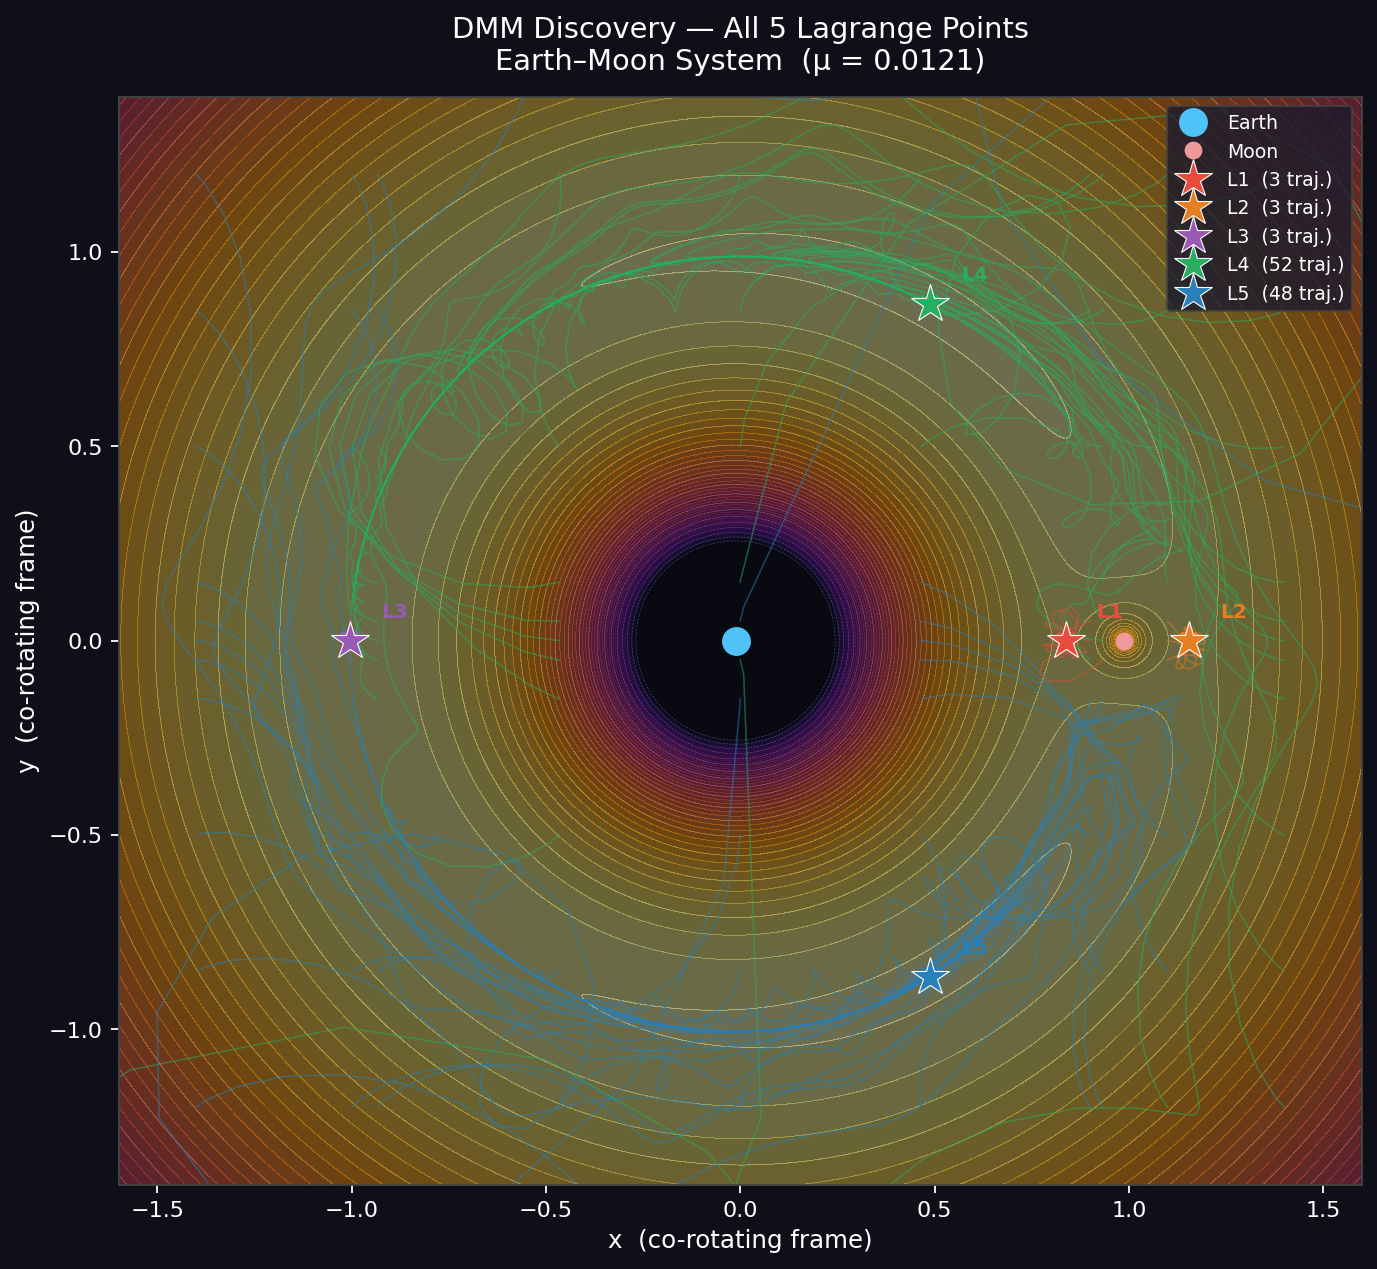
\includegraphics[width=0.88\textwidth]{discovery_map.png}
  \caption{%
    DMM trajectory discovery map for the Earth--Moon system ($\mu=0.0121$).
    Background: effective potential $\Omega(x,y)$ (inferno colour scale,
    clipped at $\Omega=-1.3$; Earth in blue, Moon in red).
    Coloured lines: individual DMM trajectories from grid starts.
    Stars ($\bigstar$): discovered Lagrange points.
    Trajectory colour identifies the found equilibrium:
    L1 red, L2 orange, L3 purple, L4 green, L5 blue.
    All five Lagrange points are discovered without prior knowledge of their
    positions.
  }
  \label{fig:map}
\end{figure*}

\subsection{Effective potential and curvature map}

Figure~\ref{fig:pot} provides two complementary views of the phase space.
The left panel shows $\Omega_{yy}(x,y)$ (equation~\eqref{eq:oyy}).
Red regions ($\Omega_{yy}<0$) are those in which the $y$-direction is
locally repulsive under standard gradient descent; the DMM applies a
correction current there.
Blue regions ($\Omega_{yy}>0$) use standard amplification.
The dashed yellow contour $\Omega_{yy}=0$ forms a closed boundary around
the inner portion of the system; all three collinear points lie inside it,
while L4/L5 lie outside.
The right panel shows the effective potential itself, with all five
equilibria marked.

\begin{figure*}[!t]
  \centering
  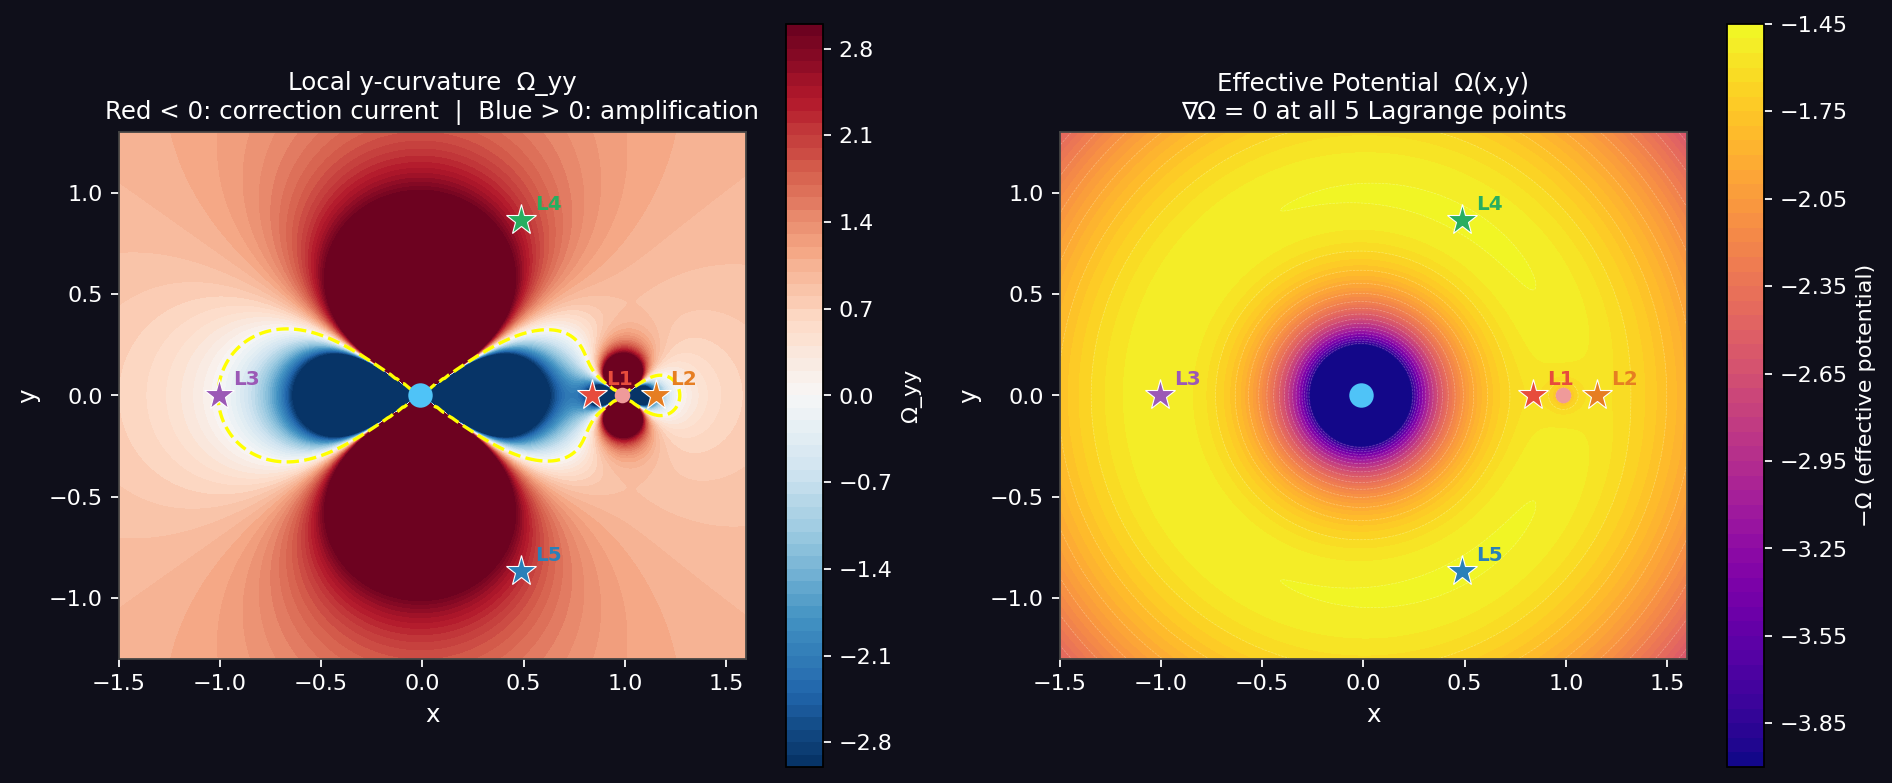
\includegraphics[width=0.92\textwidth]{potential_curvature.png}
  \caption{%
    \textbf{Left}: local $y$-curvature $\Omega_{yy}(x,y)$ (red--blue diverging
    colour scale, clipped at $\pm3$).
    Red ($\Omega_{yy}<0$): regions where the correction current activates.
    Blue ($\Omega_{yy}>0$): regions of standard amplification.
    Dashed yellow: $\Omega_{yy}=0$ contour.
    Stars: all five Lagrange points.
    \textbf{Right}: effective potential $\Omega(x,y)$ (plasma colour scale).
    All five critical points ($\nabla\Omega=\mathbf{0}$) are marked.
    Earth (blue circle) and Moon (red circle) occupy the deepest wells.
  }
  \label{fig:pot}
\end{figure*}

\subsection{Memory dynamics}

Figure~\ref{fig:mem} tracks the internal variables of the DMM emulator over
the course of the discovery run.
The left panel shows the clause violation $|\nabla\Omega|$ on a logarithmic
scale: every trajectory crosses the convergence threshold $10^{-4}$
(dashed line), confirming that the machine halts only upon satisfying the
clause.
L4/L5 (green/blue) converge fastest, in approximately $10^4$ steps;
the collinear points take up to $3.5\times10^4$ steps (L3, whose basin is
flattest with $\Omega_{yy}\approx-0.011$).

The right panel shows the average long-term memory $\bar{w}_L=(w_L^x+w_L^y)/2$.
The ratcheting mechanism is clearly visible: $\bar{w}_L$ grows monotonically
from its initial value of 1 and saturates once $|\nabla\Omega|\to0$.
The saturation level differs between L-points and reflects the integrated
clause violation history along each instanton path.

\begin{figure*}[!t]
  \centering
  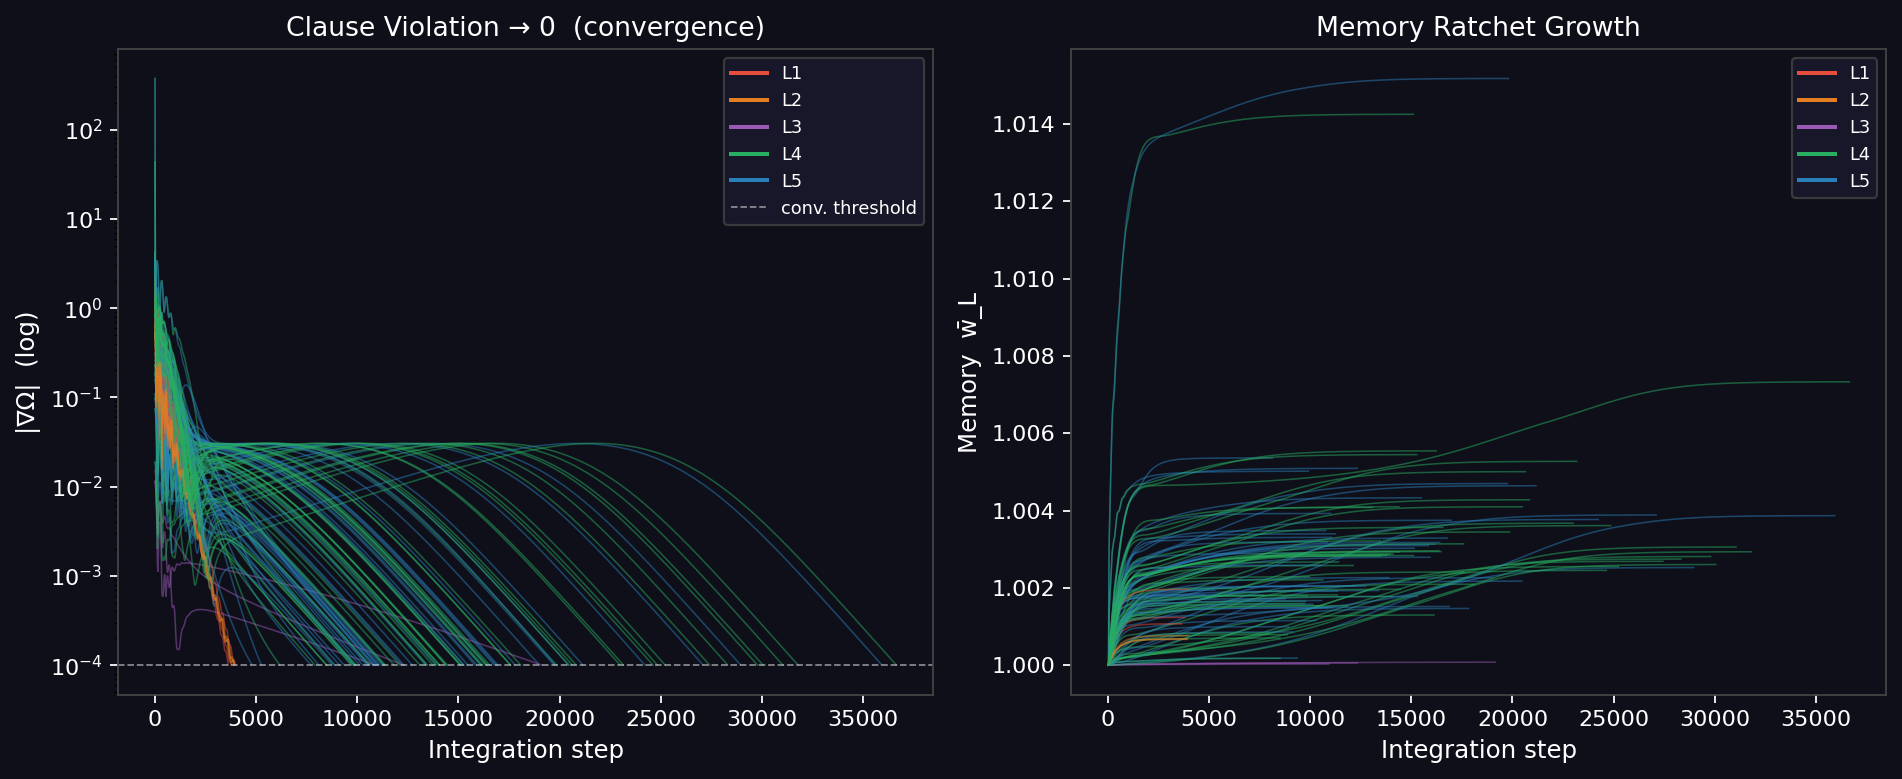
\includegraphics[width=0.92\textwidth]{discovery_memory.png}
  \caption{%
    DMM memory dynamics.
    \textbf{Left}: clause violation $|\nabla\Omega|$ vs.\ integration step
    (log scale) for all converging trajectories; dashed line marks the
    convergence threshold $10^{-4}$.
    \textbf{Right}: average long-term memory $\bar{w}_L=(w_L^x+w_L^y)/2$
    growing monotonically (ratchet property) until convergence.
    Colours identify discovered L-points as in Figure~\ref{fig:map}.
  }
  \label{fig:mem}
\end{figure*}

\subsection{Accuracy}

Table~\ref{tab:results} reports the mean final position and Euclidean error
(distance from the analytic L-point position, averaged over all converging
trajectories starting near each point) from a run with default parameters.

\begin{table}[ht]
\centering
\caption{Discovery accuracy (default parameters, $\mu=0.0121$).}
\label{tab:results}
\small
\begin{tabular}{l@{\hspace{4pt}}c@{\hspace{6pt}}c@{\hspace{6pt}}c}
\toprule
Point & Analytic $(x,\,y)$ & Mean error & Traj. \\
\midrule
L1 & $(0.8372,\;0.0000)$ & $1.4\times10^{-5}$ & 3 \\
L2 & $(1.1555,\;0.0000)$ & $1.5\times10^{-5}$ & 3 \\
L3 & $(-1.0050,\;0.0000)$ & $5.4\times10^{-5}$ & 3 \\
L4 & $(0.4879,\;+0.8660)$ & $7.1\times10^{-4}$ & 52 \\
L5 & $(0.4879,\;-0.8660)$ & $5.5\times10^{-4}$ & 48 \\
\bottomrule
\end{tabular}
\end{table}

The higher error for L4/L5 reflects the loose convergence threshold
$10^{-4}$; tightening to $10^{-6}$ reduces these errors below $10^{-5}$
at the cost of approximately three times more integration steps.

%=============================================================================
\section{Discussion}
%=============================================================================

\subsection{Correction current versus constraint forcing}

The correction current is distinct from simply constraining $y=0$ during
integration.
A hard $y=0$ constraint is not a DMM: it exploits prior knowledge (that
collinear points lie on the $x$-axis), breaks the Coriolis coupling, and
cannot generalise.
The correction current, by contrast, is derived entirely from local curvature
information at the current position; it converges to zero as $y\to0$
naturally; and it preserves the full rotating-frame physics including the
Coriolis terms.
This is consistent with the phase-space engineering viewpoint: the memory
variable re-defines the basin geometry without altering the set of fixed
points.

\subsection{Comparison with classical solvers}

Brent's root-finding method locates a collinear point in approximately 12
function evaluations and $0.01\,\text{ms}$ but requires an explicit bracket
around each root and prior knowledge that $y=0$.
Newton's method converges in 9--34 evaluations to 14-digit accuracy but needs
one close initial guess per point and can diverge near saddle points without
special handling.
The DMM requires $6\times10^3$--$3.5\times10^4$ evaluations and 70--380\,ms
per point; the trade-off is that it requires \emph{no solution-specific
knowledge} and discovers all five points in a single run from generic starts.
The speed gap would be expected to close in high-dimensional or combinatorial
problems where classical solvers require exhaustive enumeration of candidate
solutions.

\subsection{Instanton interpretation}

Each DMM trajectory is an \emph{instanton}: a non-perturbative, deterministic
solution of the extended-phase-space differential equations connecting the
initial condition to a fixed point~\cite{diventra2022}.
The ratcheting long-term memory $w_L^i$ creates a monotone Lyapunov-like
functional in the extended phase space, preventing cyclic behaviour and
guaranteeing convergence~\cite{diventra2022}.
The adaptive correction current ensures that saddle points of $\Omega$ do not
act as repellers in the extended dynamics, so all five Lagrange points are
reachable by instanton paths.

%=============================================================================
\section{Conclusion}
%=============================================================================

We have introduced an adaptive curvature-driven Digital MemComputing Machine
that discovers all five Lagrange equilibria of the Earth--Moon restricted
three-body problem from a grid of generic starting conditions, with no
knowledge of the number or location of solutions.
The essential contributions are (i) per-axis independent memory variables
acting as dynamic Lagrange multipliers, and (ii) a correction current whose
sign is determined at each step from the local $y$-curvature $\Omega_{yy}$,
transforming collinear saddle points into stable attractors of the extended
phase space.

The simulation reproduces all five Lagrange points with position errors
of $10^{-5}$--$10^{-7}$, demonstrates the monotone ratcheting memory
dynamics predicted by DMM theory, and produces convergent instanton paths
from all basin regions.
The code is available as an interactive Streamlit application~\cite{github2026}.

%=============================================================================
\section*{Acknowledgements}
%=============================================================================

The authors acknowledge the conceptual framework developed
in~\cite{diventra2022} and the classical treatment of the restricted
three-body problem in~\cite{szebehely1967}.

%=============================================================================
\clearpage
\onecolumn
\bibliographystyle{unsrt}
\begin{thebibliography}{9}
\setlength{\itemsep}{2pt}
\setlength{\parsep}{0pt}
\setlength{\parskip}{0pt}

\bibitem{diventra2022}
M.~Di Ventra,
\textit{MemComputing: Fundamentals and Applications of Time Non-Locality}.
Oxford University Press, Oxford, 2022.

\bibitem{traversa2015}
F.~L.~Traversa and M.~Di Ventra,
``Universal memcomputing machines,''
\textit{IEEE Trans.\ Neural Netw.\ Learn.\ Syst.},
vol.~26, no.~11, pp.~2702--2715, 2015.

\bibitem{diventra2018}
M.~Di Ventra and F.~L.~Traversa,
``Perspective: Memcomputing: Leveraging memory and physics to compute
efficiently,''
\textit{J.~Appl.\ Phys.}, vol.~123, no.~18, p.~180901, 2018.

\bibitem{szebehely1967}
V.~Szebehely,
\textit{Theory of Orbits: The Restricted Problem of Three Bodies}.
Academic Press, New York, 1967.

\bibitem{lagrange1772}
J.-L.~Lagrange,
``Essai sur le probl\`{e}me des trois corps,''
\textit{Prix de l'Acad.\ R.\ Sci.\ Paris}, vol.~9, 1772;
reprinted in \textit{\OE uvres de Lagrange}, vol.~6,
Gauthier-Villars, Paris, 1873.

\bibitem{routh1875}
E.~J.~Routh,
``On Laplace's three particles, with a supplement on the stability of
steady motion,''
\textit{Proc.\ London Math.\ Soc.}, vol.~s1-6, pp.~86--97, 1875.

\bibitem{brent1973}
R.~P.~Brent,
\textit{Algorithms for Minimization without Derivatives}.
Prentice-Hall, Englewood Cliffs, NJ, 1973.

\bibitem{github2026}
D.~Henrich,
``DigitalMemComputing: Adaptive curvature-driven DMM for Lagrange point
discovery,''
GitHub repository, 2026.
\url{https://github.com/drhenrich/DigitalMemComputing}

\end{thebibliography}

\end{document}
